\documentclass{beamer}
\mode<presentation>{\usetheme{AV}}
\usepackage{etex}
\usepackage[export]{adjustbox}
\usepackage{epsfig}
\usepackage{feynmp}
\usepackage{verbatim}
\usepackage{listings}
\usepackage{colortbl}

\usepackage{color}

\definecolor{mygreen}{rgb}{0,0.6,0}
\definecolor{mygray}{rgb}{0.5,0.5,0.5}
\definecolor{mymauve}{rgb}{0.58,0,0.82}

\lstset{ %
  backgroundcolor=\color{white},   % choose the background color; you must add \usepackage{color} or \usepackage{xcolor}
%  basicstyle=\footnotesize,        % the size of the fonts that are used for the code
  breakatwhitespace=false,         % sets if automatic breaks should only happen at whitespace
  breaklines=true,                 % sets automatic line breaking
  captionpos=b,                    % sets the caption-position to bottom
  commentstyle=\color{mygreen},    % comment style
  deletekeywords={...},            % if you want to delete keywords from the given language
  escapeinside={\%*}{*)},          % if you want to add LaTeX within your code
  extendedchars=true,              % lets you use non-ASCII characters; for 8-bits encodings only, does not work with UTF-8
  frame=single,                    % adds a frame around the code
  keepspaces=true,                 % keeps spaces in text, useful for keeping indentation of code (possibly needs columns=flexible)
  keywordstyle=\color{blue},       % keyword style
  language=Octave,                 % the language of the code
  morekeywords={*,...},            % if you want to add more keywords to the set
  numbers=left,                    % where to put the line-numbers; possible values are (none, left, right)
  numbersep=5pt,                   % how far the line-numbers are from the code
  numberstyle=\tiny\color{mygray}, % the style that is used for the line-numbers
  rulecolor=\color{black},         % if not set, the frame-color may be changed on line-breaks within not-black text (e.g. comments (green here))
  showspaces=false,                % show spaces everywhere adding particular underscores; it overrides 'showstringspaces'
  showstringspaces=false,          % underline spaces within strings only
  showtabs=false,                  % show tabs within strings adding particular underscores
  stepnumber=2,                    % the step between two line-numbers. If it's 1, each line will be numbered
  stringstyle=\color{mymauve},     % string literal style
  tabsize=2,                       % sets default tabsize to 2 spaces
  title=\lstname,                   % show the filename of files included with \lstinputlisting; also try caption instead of title
belowskip=-1.2em
}

\usepackage[utf8]{inputenc}
\usepackage[T1]{fontenc}
\usepackage{lmodern}
\usepackage{amsfonts}
\usepackage{supertabular}

\usepackage{textcomp}
\usepackage{amsmath}
\usepackage{amssymb}
\usepackage{graphicx}
%\usepackage{wrapfig}
\usepackage{subfigure}
\usepackage{type1cm}
\usepackage{tikz}
\usepackage{tikz-3dplot}
\usepackage{tikz}
\usepackage{tikz-3dplot}
\usepackage{pgfplots}
\usepackage{ulem}
\usetikzlibrary{shapes,arrows}
\usepackage{pgfplots}
\usetikzlibrary{shapes,arrows}
\usepackage{rotating}%     - to rotate boxes, pictures etc.
\usepackage{amsmath}%      - to use the AMS extended math package
\usepackage{amssymb}%      - to obtain additional math symbols in AMS fonts
\usepackage{amscd}%        - to obtain AMS flow chart utilities
\usepackage{array}%        - to obtain additional tabular functionality
\usepackage{multirow}%     - for multirow-entries in tables
\usepackage{supertabular}% - for multi-page tables
\usepackage{dcolumn}%      - decimal-point aligned colums in tables
\usepackage{xspace}%       - to add empty space after commands
\usepackage{upgreek}%      - provide upright greek letters
\usepackage{calc}%         - enhanced calculus in LaTeX macros
\usepackage{ifthen}%       - enhance logical structures in LaTeX macros
\usepackage{cite}%         - for multiple citations like [1-4] instead of [1,2,3,4]
\usepackage{tikz} 
%\usepackage{enumitem} 
\usepackage{multirow}
\usepackage{amssymb}
\usepackage{mathtools}
\usepackage{graphicx}
%\usepackage[dvipsnames]{xcolor}
%\input{../zeusSEC-def}










%\setbeamertemplate{navigation symbols}{}
%\setbeamertemplate{footline}[page number]{}


%\newenvironment{changemargin}[2]{%
%\begin{list}{}{%
%\setlength{\topsep}{0pt}%
%\setlength{\leftmargin}{#1}%
%\setlength{\rightmargin}{#2}%
%\setlength{\listparindent}{\parindent}%
%\setlength{\itemindent}{\parindent}%
%\setlength{\parsep}{\parskip}%
%}%
%\item[]}{\end{list}}

%\newcommand{\maxFrameImage}[1]{
%\begin{frame}[plain]
%\begin{changemargin}{-1cm}{-1cm}
%\begin{center}
%\includegraphics[width=1.0\paperwidth,height=1.0\paperheight,keepaspectratio]
%{#1}
%\end{center}
%\end{changemargin}
%\end{frame}
%}


\def\Tiny{\fontsize{4.0pt}{4.0pt}\selectfont}

\title[DPHEP2017]{2nd Data Preservation in High Energy Physics Collaboration Meeting}
\subtitle[DPHEP2017]{DPHEP2017}
\author[Andrii Verbytskyi]{
Andrii Verbytskyi
}
\date[]{\\ \today}


\setbeamersize{text margin left=.3cm,text margin right=.3cm} 
\listfiles
\begin{document}

\usebackgroundtemplate{%
  \tikz\node [anchor=north east, inner sep=0pt,opacity=0.18]  at (current page.center)
     {\includegraphics[height=0.5\paperheight,width=\paperwidth]{bkg3.eps}};
}

\frame{
%  \node [anchor=north east, inner sep=0pt,opacity=0.18]  at (current page.center)
 %    {
\includegraphics[height=0.097\paperheight,width=0.5\paperwidth]{bg}};
     
     %\begin{tikzpicture}%[remember picture, overlay]
%\end{tikzpicture}          
\vspace{0.3cm}
\begin{figure}
\includegraphics[height=1.0cm]{eps/zeus.eps}
\includegraphics[height=1.0cm]{eps/h1.eps}

\includegraphics[height=1.0cm]{eps/MPP_os_logo_cmyk.eps}

\includegraphics[height=1.0cm]{eps/DESY-Logo-cyan-RGB_ger.eps}
\hspace*{12.0cm}
\end{figure}
\begin{center}
\vspace{1.3cm}
{\LARGE The ZEUS and H1 long term data preservation projects in Max-Planck Institute f\"{u}r Physik}
\vspace{0.3cm}
\end{center}
\begin{center}
\vspace{0.3cm}
Andrii Verbytskyi\\
\end{center}
\vspace{1.0cm}
\begin{center}
\footnotesize  2nd Data Preservation in High Energy Physics Collaboration Meeting \\Geneve,\\ \today
%\footnotesize  24th International Workshop on Deep-Inelastic Scattering and Related Subjects\\Hamburg,\\ \today
\end{center}
\vspace{0.4cm}
}




\usebackgroundtemplate{%
  \tikz\node [anchor=north east, inner sep=0pt,opacity=0.18]  at (current page.center)
     {\includegraphics[height=1.0\paperheight,width=\paperwidth]{eps/desy-1}};
}


\frame{\frametitle{HERA data preservation motivation}
\begin{itemize}
\item Future data (re-)analysis with new models and new approaches.
\item Modelling for the future experiments.
%\item Outreach and education.
\end{itemize}

\vspace{1cm}
HERA reminder:
\begin{itemize}
\item The only $e^{\pm}p$ collider, 1991-2007;
\item $27.5GeV$ $e^{\pm}$; $460,575,820,920GeV$ $p$;
\item (Un)polarized $e^{\pm}$ collide with $p$; 
\item Polarised $e^{\pm}$ collide with $H/D/.../Xe$ targets;
\item $p$ collide with nuclear targets.
\end{itemize}

{\bf Two complementary active sides for the HERA data preservation: DESY (covered by Achim) and MPP. }
}


\usebackgroundtemplate{}




\frame{\frametitle{MPP model for DPHEP }
{\bf Data preservation is about  new and interested results with old data.}\\
We describe  ingredients and tools:
\begin{columns}[c]
\column{0.4\linewidth}
\begin{itemize}
\item Data bits
\item Software
\end{itemize}
\column{0.6\linewidth}
\begin{itemize}
\item Experiment documentation
\item DP policies and  documentation
\end{itemize}
\end{columns}

\begin{itemize}
\item But in the end we are interested in {\bf physics }.
%\item We are not interested in: {\bf Tools}  -- files, storages, clusters, systems etc.
%There are people in Max Planck Computing and data facility (MPCDF) who deal much better with these things.
\end{itemize}
Brief idea: enable physics and make it doable with modern methods in modern environments with minimal effort.\\
%{\bf Follow modern approaches is helpful.}
%The talk will describe some tools\dots but only with an intention to show how these {\bf serve science.}% were made irrelevant!}\\
%\vspace{1cm}

}


\frame{\frametitle{MPP model for bits preservation}
MPP bits preservation is similar to approach from DESY.\\
The main differences comes from the ideas to
\begin{itemize}
\item Enable option for worldwide access via Grid.
\item Study options to benefit from larger Data Preservation efforts.
\end{itemize}
}


\frame{\frametitle{MPP model for documentation preservation and policies}
MPP data preservation relies on the documentation preserved by DESY/DESY library/InSpire.\\
The main idea is to provide the missing or DPHEP@MPP-specific documentation:
\begin{itemize}
\item Access to data in MPCDF (H1 and ZEUS).
\item Monte Carlo generation procedures, event display usage, database of data samples, virtual machine usage (ZEUS). 
\end{itemize}

The policies on the data/documentation access  are same as in DESY: defined by collaboration spokespersons.

}


\frame{\frametitle{MPP model for software preservation}
MPP software preservation is different from DESY.\\
Explicit effort put to make software it work in the next 10-15 years.
\begin{itemize}
\item Rely on industry, not HEP-only standards.
\item Enable integration and compatibility with new physics software, e.g. data bases and Monte Carlo generators.
\end{itemize}
Main focus was on ZEUS software:
no recompilation of software, but frozen environment that can be installed on virtual or real machine is provided:
ISO image of full operating system relying on Intel $x86$  architecture.
Though not implemented, same approach is applicable to H1.

}





\frame{\frametitle{ \   }
\begin{center}{\Huge ZEUS}\end{center}
}



\frame{\frametitle{ZEUS analyses statistics}
The results of recent yeas are produced in Data Preservation mode.
\begin{itemize}
\item 1X papers since 2014
%\item  3 this year!
\item  active analyses, more results on the way.
\end{itemize}
}




\frame{\frametitle{ZEUS data bits in MPP}
\begin{itemize}
\item  ZEUS data are stored in MPCDF on locally accessible tapes and in disk pool.
\item Access via multiple protocols with grid tools worldwide to disk pools..
\item Grid-enabled storage for new samples (Monte Carlo) and analysis is available.
\item Straightforward procedure to update or add new samples.
\item Stored part of private Ntuples/analyses directly in MPP.
\item Future:  keep only most important bits in disk pool and have a mechanism to get the other data if needed.
%\item Newest MC samples produced in 2015-2016 are in MPCDF only (so far).
\end{itemize}
%{\bf H1 and ZEUS data is treated equaly.}
}


%\footnote{Because of data reshiffling now H1 data temporary is only on tape}	


\frame{\frametitle{ZEUS data in MPP and DESY: Bits statistics}
Data content is simple ROOT and PAW ntuples (see talk from Achim).
Logs and some inputs for Monte Carlo simulation are available.\\
\hspace{6cm}\begin{table}\centering\bf\begin{tabular}{|c|c|c|}\hline

{\color{maroon}           } & {\color{maroon}   MPCDF     }&{\color{maroon} DESY }          \\\hline\hline
{\color{maroon}Files:      }&{\color{maroon}   1.2M           }&{\color{maroon}  1.1M             } \\
{\color{maroon}Volume:     }&{\color{maroon}   $250T$           }&{\color{maroon}  $>250T$             } \\
{\color{maroon}Work area:  }&{\color{maroon}    yes       }&{\color{maroon} yes,limited           } \\
{\color{maroon}Access:     }&{\color{maroon}   Worldwide  }&{\color{maroon} DESY          } \\
{\color{maroon}Protocols: } &{\color{maroon}   Multiple, see list   }&{\color{maroon} NFS mount     } \\
{\color{maroon}Auth:      } &{\color{maroon}   Grid certificate }&{\color{maroon} DESY account  } \\\hline

\end{tabular}
\end{table}

Available at:
\begin{itemize}
\item gsidcap://grid-srm.rzg.mpg.de:22128/pnfs/rzg.mpg.de/data/zeus
\item grid-gftp2.rzg.mpg.de 
\item davs://grid-dav.rzg.mpg.de:2880//zeus
\item \dots
\end{itemize}

}



\frame{\frametitle{Documentation and documentation preservation in MPP}
As most documentation is  available in InSpire and DESY sites,
MPP covers the missing parts:
\begin{itemize}
\item Instructions on data access
\item Up-to dated database of available samples
\item Instructions for Monte Carlo generation and reconstruction
\end{itemize}

Available at: https://wwwzeus.mpp.mpg.de/dphep.html


%{\bf Promised to link to ZEUS analysis web page.}

}





\frame{\frametitle{ZEUS software in MPP}
\begin{itemize}
\item Main software for the analysis is vanilla ROOT.
\item Additional software includes:
\begin{itemize}
\item ZEVIS, the event display based on ROOT;
\item CNINFO, the event data base, based on ROOT and SQLite3;
\item ZMCSP Monte-Carlo standalone generation packages -- see next slides.
\end{itemize}
\item +any ROOT extension that will work for you\dots
\end{itemize}

%\begin{figure}
%\hspace*{1.0cm}
\begin{columns}[c]
\column{0.49\linewidth}
\adjincludegraphics[height=5.0cm, trim={ {0.5\Width}  {0.00\Width}    {0.0\Height}   {0.0\Height}}, clip=true]{eps/analysis.eps}
\column{0.49\linewidth}

\includegraphics[width=5.0cm]{eps/rootlogo.eps}\\

\includegraphics[width=2.0cm]{eps/sqlite370_banner.eps}
 {\cal{ + your favourite software e.g. FastJet }}
\end{columns}

}



\frame{\frametitle{ZEUS software environment/VM}
A certain environment is needed  for the analysis, i.e. DESY NAF or MPP/MPCDF machines are working well now.
%As of 2017 the demands are low and easy to fulfil: 
%\begin{itemize}
%\item Both DESY and MPP/MPCDF provide an access to a batch computing cluster.
%In many cases it is enough for basic tests and analysis.
%\end{itemize}
In parallel:% But what about 2020+?
\begin{itemize}
\item Virtual machines(VM) are a very attractive {\bf long-term} solution;
\item The way other experiments (LEP/LHC) are going;
\item The solution has very generic requirements, will survive for a long time.
\end{itemize}
%Because of very generic requirements it is foreseen that both environments will 
%remain functional for a long time.
}


%\usebackgroundtemplate{%
%  \tikz\node [anchor=north, inner sep=0pt,opacity=0.18,xshift=2cm]  at (current page.center)
%     {\centering
\includegraphics[width=0.5\paperwidth]{eps/iso-image}
\includegraphics[width=0.5\paperwidth]{eps/MPP_os_logo_cmyk}
%     };
%}

\frame{\frametitle{ZEUS software environment/VM}
Vitalisation for ZEUS has a two-fold purpose: it provides  {\bf benchmark } environment that suppose to work 
for a long time and it can be used, if desired, as a {\bf super-portable production environment}.\\
It is based on DVD ISO image with SL7 and all software. It has options for:
\begin{itemize}
\item Automatic install on virtual or real hardware;
\item Customisation, root privileges, etc.;
\item Unlimited number of installations $\rightarrow$ potentially usable on clouds;
\item Usage not restricted to any laboratory or virtualization software. Can run anywhere.
\item {\bf Tested by $\approx 5$ users, found to be stable and easier to use than other options.}
\end{itemize}

%It is not necessary to use it in the production if something more productive like institute's cluster 
%is working for you.

}

\usebackgroundtemplate{}


\frame{\frametitle{ZEUS software environment/VM}
VM includes:
\begin{itemize}
\item ZEUS software: ROOT, MC simulation, event display, file catalogue, setup scripts etc.
\item Modern MC generators, FastJet, cernlib, PAW,  Rivet and other popular and ``not really'' packages.
\item Anything you will want to install\dots
\item Available at: https://wwwzeus.mpp.mpg.de/dphep.html together with  documentation and video tutorials. 
\item Agree access and download it.
\end{itemize}
%\begin{figure}\centering
%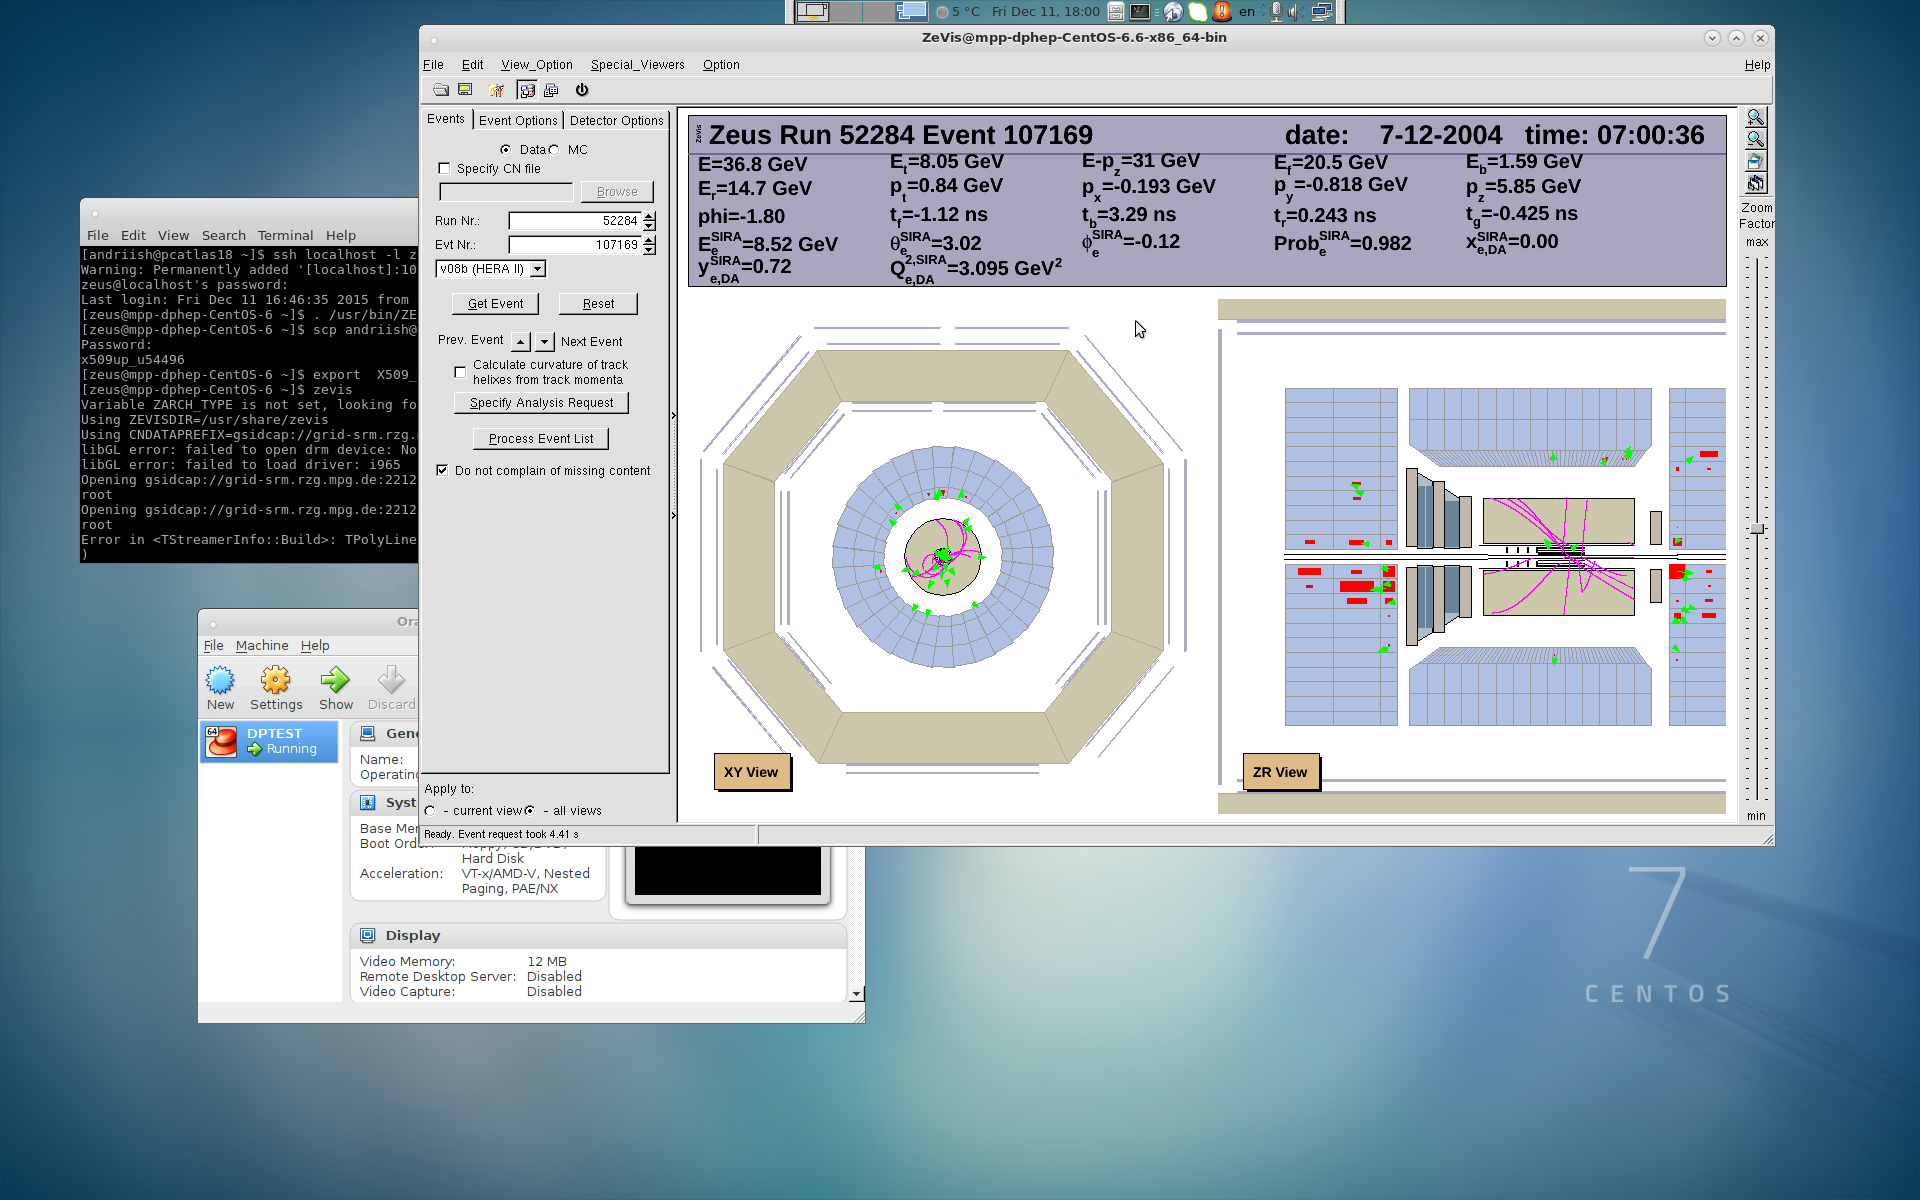
\includegraphics[height=0.5\textheight]{eps/Screenshot_2.eps}
%\end{figure}

}

\frame{\frametitle{Data preservation for ZEUS: Software environment/VM}
\begin{figure}\centering
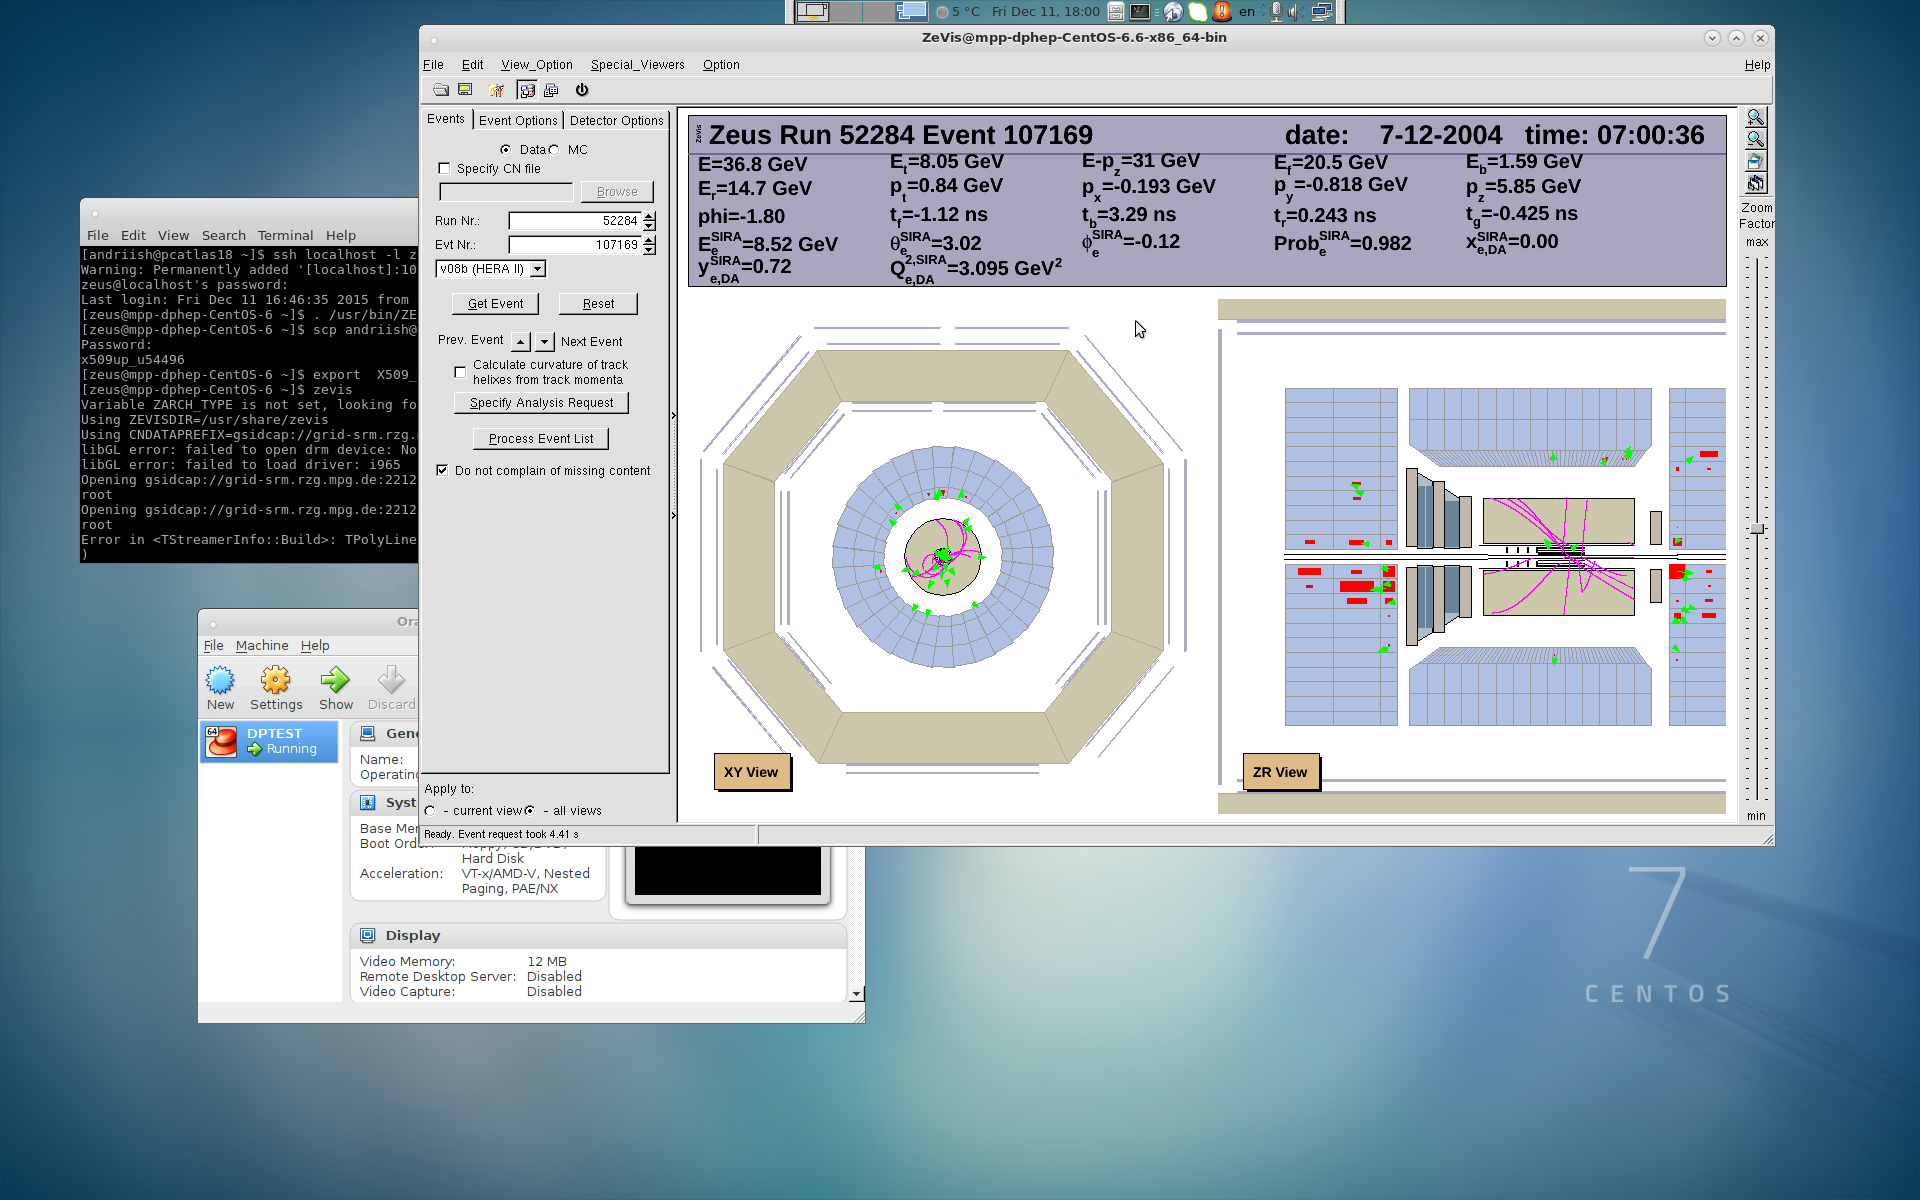
\includegraphics[width=1.0\textwidth]{eps/Screenshot_2.eps}
\end{figure}
}

\frame{\frametitle{Monte Carlo production}
%\frame{\frametitle{Motivation for the MC generation}
%An elaborated dish in the cookbook is the recipe for the Monte Carlo simulations.\\
Motivation:\\
\begin{itemize}
\item Some analyses require more MC that is not available;
\item Some analyses can be significantly improved with new MC;
\item New MC generators/models can be tuned;
\item New experiments can use it for the technical studies.
\end{itemize}



}



\frame{\frametitle{The MC recipe ingredients}
\begin{itemize}
\item Instruction to generate events with old ZEUS generators are prepared.
\item An interface to modern HEP event records based on HepMC3 libray is developed.
  ZEUS MC  can be produced from with modern MC generator, e.g.\ NLO capable SHERPA+BlackHat.
\item ZMCSP (ZEUS Monte Carlo Standalone Package) is a tarball with  all the software needed for the reconstruction
of MC simulated events. It has no external dependencies, runs on modern Grid clusters, virtual machine, a laptop.
On the Grid it can produce 50-100M events\footnote{ZEUS has 360M of data events} per week. 
Supplemented with example of scripts and documentation.
%\item The first two samples were generated this summer. See Iurii's talk.
%It was found that the key to success is to {\bf read and follow the instructions}.
%\item There is a lot of computing resources around, where it is possible to generate even large samples.
%20-50-100M events is NOT a problem. 
%\item In practice the generation with new MC generators is not much complicated, however only tiny samples were produced with
%SHERA 2.2 and blackhat 0.9.9.
\end{itemize}
}

\frame{\frametitle{The MC generation: SHERPA+BlackHat multijet setup}
\begin{figure}\centering
\includegraphics[width=0.4\linewidth]{kt.eps}
\includegraphics[width=0.4\linewidth]{nt.eps}
\end{figure}
Pseudorapidity distribution of jets with $k_{T}(R=1.0)$  algorithm applied in in lab. frame  (left),
track multiplicity (right) with SHERPA+BlackHat MC simulated sample.
}


\frame{\frametitle{The MC generation}
\begin{itemize}
\item So far two analyses used the available option of MC generation at least to some extend.
\item No modern generators at the moment, but the option is attractive, especially for precision measurements.
\end{itemize}
}



\frame{\frametitle{ \   }
\begin{center}{\Huge H1}\end{center}
}



\frame{\frametitle{H1 statistics}
The results of recent yeas are produced in Data Preservation mode.
\begin{itemize}
\item 1X papers since 2014
%\item  3 this year!
\item  active analyses, more results on the way.
\end{itemize}
}



\frame{\frametitle{H1 data in MPP and DESY: Bits statistics}



\hspace{6cm}\begin{table}\centering\bf\begin{tabular}{|c|c|c|}\hline

{\color{maroon}           } & {\color{maroon}   MPCDF     }&{\color{maroon} DESY }          \\\hline\hline
{\color{maroon}Files:      }&{\color{maroon}   XM           }&{\color{maroon}  XM             } \\
{\color{maroon}Volume:     }&{\color{maroon}   $XT$           }&{\color{maroon}  $>XT$             } \\
{\color{maroon}Work area:  }&{\color{maroon}    yes       }&{\color{maroon} yes,limited           } \\
{\color{maroon}Access:     }&{\color{maroon}   Worldwide  }&{\color{maroon} DESY          } \\
{\color{maroon}Protocols: } &{\color{maroon}   Multiple, see list   }&{\color{maroon} NFS mount     } \\
{\color{maroon}Auth:      } &{\color{maroon}   Grid certificate }&{\color{maroon} DESY account  } \\\hline

\end{tabular}
\end{table}

Available at:
\begin{itemize}
\item gsidcap://grid-srm.rzg.mpg.de:22128/pnfs/rzg.mpg.de/data/hone
\item grid-gftp2.rzg.mpg.de 
\item davs://grid-dav.rzg.mpg.de:2880//hone
\item \dots
\end{itemize}

}



\frame{\frametitle{H1 software in MPP}
Don't have specific setup, just same as in DESY (see Achim's talk). Briefly:
\begin{itemize}
\item Main software for the analysis is ROOT with many H1 specific classes. Large part of analysis information is available with vanilla ROOT.
\item Huge effort by H1 Collaboration to ensure software can be compiled relatively easy on new systems.
%\item 
\end{itemize}
}


\frame{\frametitle{H1 documentation in MPP}
As most documentation is  available in InSpire and DESY sites,
MPP covers the missing parts:
\begin{itemize}
\item Instructions on data access in MPP, which is the same as for ZEUS
\end{itemize}
Available at: https://wwwzeus.mpp.mpg.de/dphep.html
}




\frame{\frametitle{Option for H1 software environment/VM}
The approach of virtualization can be extended to H1, as the basic software it the same.
\begin{itemize}
\item ROOT, compilers, libraries, etc.
\item Modern MC generators, FastJet, cernlib, PAW,  other HEP packages.
\end{itemize}
}






%\frame{\frametitle{What do we have}
%\begin{itemize}
%\item Full MC simulation and reconstruction chain is preserved in ZMCSP,
%{\bf ZEUS Monte Carlo Standalone package}.
%The input comes in ADAMO format, the output are the Common Ntuples.
%By J.M.\&A.V.
%\item formoza, an utility that converts HEPEVT-like event records (ZEUS HEPEVT) to 
%ADAMO format. By Y.G.
%\item HepMC3 library that can convert HepMC event records to other event records, including 
%these readable by ZM
%\end{itemize}
%}







%\frame{\frametitle{Theory of MC generation: how does it work}
%\begin{itemize}
%\item {With an old generator:
%\begin{itemize}
%\item Run it using the old ZEUS steering cards.
%\end{itemize}%
%}


%\item {With a new generator:
%\begin{itemize}
%\item Set-up the generator, to produce events in HepMC format.
%\item Convert the output to HEPEVT-like event record with HepMC3 library.
%\item Convert the HEPEVT-like event records to ADAMO  using formoza.
%\end{itemize}
%}
 
%\item Rename the resulting files according to  the desired trigger periods.
%\item Use the renamed files as an input for ZMCSP package.
%\end{itemize}
%The detailed instructions for every step are in the Data Preservation paper and
%ZEUS Data Preservation page in MPP. https://wwwzeus.mpp.mpg.de/dphep.html
%}



%\frame{\frametitle{Practice of MC generation: How does it work}
%\begin{itemize}
%\item The first two samples were generated this summer. See Iurii's talk.
%It was found that the key to success is to {\bf read and follow the instructions}.
%\item There is a lot of computing resources around, where it is possible to generate even large samples.
%20-50-100M events is NOT a problem. 
%\item In practice the generation with new MC generators is not much complicated, however only tiny samples were produced with
%SHERA 2.2 and blackhat 0.9.9.
%\end{itemize}
%}




%\frame{\frametitle{Problems of MC generation}
%\begin{itemize}
%\item The validation of output relays on the tests that were performed by J.M.
%It is recommended to do them for every particular MC generation setup. The MC input was deleted, but some samples survived $\rightarrow$ should be tested very soon.
%\item It was not discussed how to store the generated samples and documentation.
%Technically everything prepared for that. The plan is to
%produce a small CNINFO database for newly generated samples and store them in MPP (MPCDF). Very small amount of work.
%\end{itemize}
%}


\section{Conclusions}

\frame{\frametitle{MPP Data Preservation summary}
\begin{itemize}
\item Data is accessible in DESY and MPCDF for H1 and ZEUS.
%\item Some data is on the tapes only and is not accessible directly.
%\item An option for full re-reconstruction is under investigation.
%\item Documentation is stored in DESY library/Inspire/web-server;
%\item Analysis requires only standard software;
%\item Software requirements are unknown.
\item An option for MC production with new and old MC generators exists for ZEUS and tested. 
Potentialy useful for H1 as well.
\item Virtualization option is implemented for ZEUS. Potentialy useful for H1 as well.
\end{itemize}
\begin{figure}\centering
\includegraphics[height=2cm]{eps/zeus.eps}
\includegraphics[height=2cm]{eps/h1.eps}
\end{figure}
}

\section{Data Preservation applications}

\frame{\frametitle{Use cases for HERA data}
\begin{itemize}
\item Something that now we are not aware about.
\item {QCD: \begin{itemize}
\item Proton structure, e.g. $F_2$ and $F_L$, strangeness in the proton;
\item Diffraction, e.g. combination of measurements;
\item Jets and event shapes with NNLO;
\item Photon structure, instantons, pentaquarks, etc.
\end{itemize}
}
\item {EW physics:\begin{itemize}
\item Prompt photons;
\item Electroweak couplings.
\end{itemize}
}
\end{itemize}
See arXiv:1601.01499 and arXiv:1512.03624  for details.
}


\usebackgroundtemplate{}


\usebackgroundtemplate{%
  \tikz\node [anchor=north, inner sep=0pt,opacity=0.18,xshift=2cm]  at (current page.center)
     {\centering\includegraphics[width=1.0\paperwidth]{eps/hermesdetector}
     };
}

\usebackgroundtemplate{}



%\frame{\frametitle{ \   }
%\begin{center}{\Huge BACKUPS}\end{center}
%}


%\frame{\frametitle{Problems and solutions in DP mode of analyses}
%Main problems with analysis of data 10+ years after end of data taking and potential solutions:
%\begin{itemize}
%\item Lack of knowledge about data existance $\rightarrow$ data discoverability, promotion, easy technical acces to data.
%\item Lack of knowledge for what the data can be used in the next generations of physicists
%$\rightarrow$ provide list of examples (e.g. arxiv:1601.01499), precise measurements are the first candidates because of guarantied result.
%\item Lack of manpower $\rightarrow$  master students with intensive supervision, i.e. up to a preprint/publication.
%\item Lack of time $\rightarrow$ eneble projects should be not more than 1 year long.
%\item Lack of documentation on simplest technicalities  $\rightarrow$  an internal documentation on the data preservation should be done.
%\item Incompatibilities of moden and 10+ y.o. analysis techniques $\rightarrow$ use them.
%\end{itemize}
%{\bf There is no way someone starts an analysis as a bachalor/master student and has an acces to data 
%on two machines in remote institute, waits for 4 month for a Monte Carlo sample to be copied, uses outdated tools that are not used anymore etc.}
%{\bf Fast and modern!}


%}







\end{document}

